\chapter{Projektmanagement}

\section{Allgemeines}

\section{Projektmanagement}
\label{projektmanagement}
Wir verwendeten die agile Projektmethologie Scrum\footnote{\url{http://www.scrum.org}} und arbeiteten dabei während 12 Wochen (4 Sprints à 3 Wochen pro Sprint).
Für diese Studienarbeit werden 8 ECTS-Punkte vergeben, wobei 1 ECTS-Punkt 30 Stunden Arbeitsaufwand bedeuten.
Dies ergibt 240 Stunden pro Person, was etwas mehr als 2 Arbeitstagen pro Woche entspricht.

Als Ausgangslage haben wir 12 Storypoints pro Sprint angenommen, wobei 1 Storypoint ungefähr einem Arbeitstag entspricht. Bis zum Schluss hat sich dieser Wert nicht merklich verändert.

% Kickoff
\subsection{Kickoff}
Das Projekts wurde mit einem Kickoff-Meeting zusammen mit dem Betreuer und dem Industriepartner am 23. Februar 2012 gestartet. Darin wurden nebst der Aufgabe auch alle Formalitäten der Arbeit besprochen. Es wurde fest gelegt, dass neben dem theoretischen Teil der Arbeit über Google Fusion Tables auch drei Anwendungsfälle aus dem GIS-Bereich umgesetzt werden sollen.

% Sprint 1
\subsection{Sprint 1}

Der erste Sprint stand ganz im Zeichen des Ausprobierens. Es ging uns darum mit dem Google Fusion Tables API bekannt zu werden. Daneben musste noch unsere Infrastruktur eingerichtet werden. Dazu zählt das Repository, unser Projektmanagement-Tool und der Build-Server.

Alle Informationen zum Sprint 1 sind auch in unserem Wiki zu finden:
\url{http://redmine.rdmr.ch/redmine/projects/gftprototype/wiki/Sprint_1}

\subsubsection{Hauptaufgaben / Fokussierung im Sprint}

\begin{itemize}
	\item Aufsetzen der Infrastruktur (Repository, Projektmanagement, Entwicklungsumgebung, Server)
	\item Einarbeitung in die Thematik
	\begin{itemize}
		\item GIS
		\item Google Fusion Tables (GFT)
		\item allenfalls weitere APIs
	\end{itemize}
	\item Erarbeitung eines ersten Roundtrips um Daten von und zu Google Fusion Tables zu schicken/empfangen
	\item Projektsetup
	\begin{itemize}
		\item GitHub\footnote{\url{http://www.github.com}} als Repository
		\item LaTex\footnote{\url{http://www.latex-project.org}} für Dokumentation
		\item Jenkins \footnote{\url{http://jenkins-ci.org}} für Continuous Integration (CI)
		\item Redmine \footnote{\url{http://www.redmine.org}} für Projektmanagement/Wiki/Bugtracker
		\item Scrum als Methodik
	\end{itemize}
\end{itemize}

\subsubsection{Ziele}
\begin{itemize}
	\item Google Fusion Table API kennen lernen, Potential abschätzen können
	\item Erster Prototyp mit GFT bauen (Roundtrip mit CRUD-Operationen)
\end{itemize}

\subsubsection{Abgabe / Deliverables}
Wir sind im ersten Sprint gut vorangekommen und konnten mit zahlreichen aufeiander aufbauenden Beispielen lernen wie das API funktioniert und welche Möglichkeiten es bietet: Abfragen erstellen, Zugriff via API, Zugriff via Google Maps Layer (FusionTablesLayer).

\begin{itemize}
	\item Repository, Build-Server und Projekmanagement-Tool aufgesetzt (siehe Kapitel \ref{infrastruktur})
	\item Lauffähiger Prototyp mit Unit-Test für CRUD-Operationen
	\item Zahlreiche Beispiele um die Funktionsweise des APIs zu testen
\end{itemize}

\subsubsection{Probleme}
Es ist uns nicht gelungen den Roundtrip zu erstellen, d.h. Daten vom Benutzer in Fusion Tables zu speichern und dies dann wieder abzufragen. Wie sich herausgestellt hat, müssen schreibende Zugriffe authorisiert sein. Dazu empfiehlt Google OAuth zu benutzen. Diese Thematik war schlicht zu gross um im ersten Sprint anzuschauen. Die schreibenden Zugriffe sind denn auch Ziel für den 2. Sprint geworden. 

% Sprint 2
\subsection{Sprint 2}

Im zweiten Sprint gab es 2 Schwerpunkte: zum einen mussten wir uns langsam Gedanken machen, welche Use Cases wir mit den Google Fusion Tables abdecken wollen. Aus diesen Use Cases sollen dann unabhängige Applikationen entstehen, welche so dann das Potential des Produktes aufzeigen sollen. Zum anderen gab es noch ein wichtiges technischen Thema, nämlich die Schreiboperationen. Dazu waren einige Grundlagen von OAuth nötig, so dass wir dann die ganze Bandbreite der Schnittstelle nutzen konnten.

Als Nebenthema mussten wir uns noch um den Import von verschiedenen GIS Dateien in Fusion Tables kümmern. Zum einen ist dies ein sehr relevantes Thema um eine Migration zu ermöglichen, zum anderen sind viele Daten in beliebigen Formate verfügbar, welche wir natürlich gern als Testdaten nutzen möchten.

Alle Informationen zum Sprint 2 sind auch in unserem Wiki zu finden:
\url{http://redmine.rdmr.ch/redmine/projects/gftprototype/wiki/Sprint_2}

\subsubsection{Hauptaufgaben / Fokussierung im Sprint}
\begin{itemize}
	\item Use Cases erarbeiten
	\item GIS Daten in GFT importieren
	\item Informationen über das \emph{Trusted Tester API} sammeln
	\item Schreiboperationen (INSERT/UPDATE/DELETE) auf Fusion Tables durchführen können (Authentifizierung mit OAuth notwendig)
\end{itemize}

\subsubsection{Ziele}
\begin{itemize}
	\item Finden von WebGIS Use Cases (1 \emph{grosser} und 2 \emph{kleine} Use Cases)
	\item Implementation eines kleinen Use Cases
	\item Geo-Daten importieren und verknüpfen
	\begin{itemize}
		\item KML importieren
		\item Converter einsetzen, dann importieren
		\item Verschiedene Fusion Tables joinen/mergen
	\end{itemize}
	\item Trusted Tester API
	\begin{itemize}
		\item Zugriff erhalten
		\item API testen
	\end{itemize}
\end{itemize}

\subsubsection{Abgabe / Deliverables}
Als ersten umzusetzenden Use Case haben wir uns für \emph{WorldData} (Kapitel \ref{worlddata}) entschieden. Zudem haben wir einen Build-Job (Kapitel \ref{converter-build}) erstellt, welcher es uns erlaubt auf einfache Art und Weise GIS Daten zu importieren.

Für OAuth haben wir ein Beispiel entwickelt, welches es einem Benutzer ermöglicht seine Tabellen für unsere Applikation freizugeben, so dass dann Schreiboperationen möglich werden.

\begin{itemize}
	\item Erster umgesetzter Use Case
	\item Import-Verfahren für GIS Daten
	\item Erweiterte GftLib (Schreiboperationen, Authentifizierung mit OAuth)
\end{itemize}

\subsubsection{Probleme}
Der Converter-Build war noch nicht sehr ausgereift, so war es noch nicht möglich das Koordinationsystem zu wechseln und überhaupt ein anderes Format zu wählen als GFT.

Bei der Authentifizierung gab es noch einige Probleme um diese für die Library nutzbar zu machen. Für den Fall, dass wir Google Fusion Tables nicht dazu verwenden möchten auf die Tabellen eines Benutzers zuzugreifen, sondern als Backend-Datenbank zu verwenden, gab es noch keine Lösung.

% Sprint 3
\subsection{Sprint 3}

Im dritten Sprint war das Hauptziel die Umsetzung des zweiten Use Cases \emph{FixMyStreet} als mobile WebApp. Dies beinhaltete unter anderem auch die Anbindung des Sencha Touch Frameworks an die Google Fusion Table.
Zusätzlich wollten wir noch einen Converter-Build erstellen, mit welchem es möglich ist verschiedenste GIS-Formate in eine Google Fusion Table zu importieren oder in andere Formate zu konvertieren.

Alle Informationen zum Sprint 3 sind auch in unserem Wiki zu finden:
\url{http://redmine.rdmr.ch/redmine/projects/gftprototype/wiki/Sprint_3}

\subsubsection{Hauptaufgaben / Fokussierung im Sprint}
\begin{itemize}
	\item Zweiter Use Case \emph{FixMyStreet} implementieren
	\item Converter-Build erstellen
\end{itemize}

\subsubsection{Ziele}
\begin{itemize}
	\item Lauffähige App für \emph{FixMyStreet} Use Case
	\begin{itemize}
		\item Eintragen von \emph{Defekten}
		\item Anzeigen der Defekte auf Karte
		\item Daten von GFT lesen / in GFT schreiben
	\end{itemize}
\end{itemize}

\subsubsection{Abgabe / Deliverables}
\begin{itemize}
	\item WebApp \emph{FixMyStreet} (erste Version)
	\item Converter-Build (GIS Formate konvertieren bzw. in GFT importieren)
\end{itemize}

Am Ende dieses Sprints hatten wir eine lauffähige Version der \emph{FixMyStreet}-WebApp (Kapitel \ref{fixmystreet}). Diese beinhaltete die Anbindung einer Google Fusion Table als Datenbank. Es sind aber noch einige kleine Bugs vorhanden, welche im nächsten Sprint korrigiert werden müssen.

\subsubsection{Probleme}
In der App sind noch einige Bugs in Bezug auf das Lesen und Schreiben der Google Fusion Table vorhanden. Es scheint als gäbe es Probleme mit der internen und externen ID der Datensätze. Zudem wurde bei verschiedenen Tests noch einige Usability-Probleme festgestellt, welche noch behoben werden müssen.

% Sprint 4
\subsection{Sprint 4}

Im letzten Sprint ging es noch um das finalisieren aller Arbeiten. Dies beinhaltete die Behebung der im Sprint 3 gefundenen Probleme in der \emph{FixMyStreet}-WebApp. Der grösste Teil der Zeit wurde aber für das Schreiben der Dokumentation eingeplant. 

Alle Informationen zum Sprint 4 sind auch in unserem Wiki zu finden:
\url{http://redmine.rdmr.ch/redmine/projects/gftprototype/wiki/Sprint_4}

\subsubsection{Hauptaufgaben / Fokussierung im Sprint}
\begin{itemize}
	\item Finalisierung aller Arbeiten
	\begin{itemize}
		\item Fertiggestellung des Use Cases \emph{FixMyStreet}
		\item Abschluss der Dokumentation
		\item Erstellung des Posters A0
	\end{itemize}
\end{itemize}

\subsubsection{Ziele}
\begin{itemize}
	\item Finalisierung des \emph{FixMyStreet} Use Cases
	\begin{itemize}
		\item Bugs / Usability-Probleme beheben
		\item Live-Daten anzeigen
		\item Berechtigungen für Benutzer
	\end{itemize}
	
	\item Finalisierung Dokumentation der Ergebnisse
	\begin{itemize}
		\item Converter-Build
		\item Use Cases / Examples
		\item Google Fusion Tables allgemein
	\end{itemize}
\end{itemize}

\subsubsection{Abgabe / Deliverables}
\begin{itemize}
	\item Dokumentation
	\item A0 Poster
	\item Vollständige Arbeit (Source Code usw.)
\end{itemize}

Nach diesem Sprint ist die Abgabe der kompletten Arbeit fällig. Dies bedeutet, dass zu diesem Zeitpunkt alle Use Cases lauffähig sind und die Dokumentation abschlossen ist. 

\section{Projektmonitoring}

\subsection{Projektverlauf}
In Abbildung \ref{overall_stories_gantt_chart} sind alle erledigten Stories mit Start- und Endpunkt auf der Zeitachse abgebildet. Leider werden die Sprints etwas verfälscht dargestellt, da wir einzelne bereits begonnene Stories aus Zeitgründen von einem Sprint in den nächsten verschoben haben (Stories \#25, \#113 und \#186). Diese werden von Redmine dann über mehrere Sprints hinweg dargestellt, was natürlich auch den Sprint künstlich "`verlängert"'.

\begin{figure}[H]
	\centering
	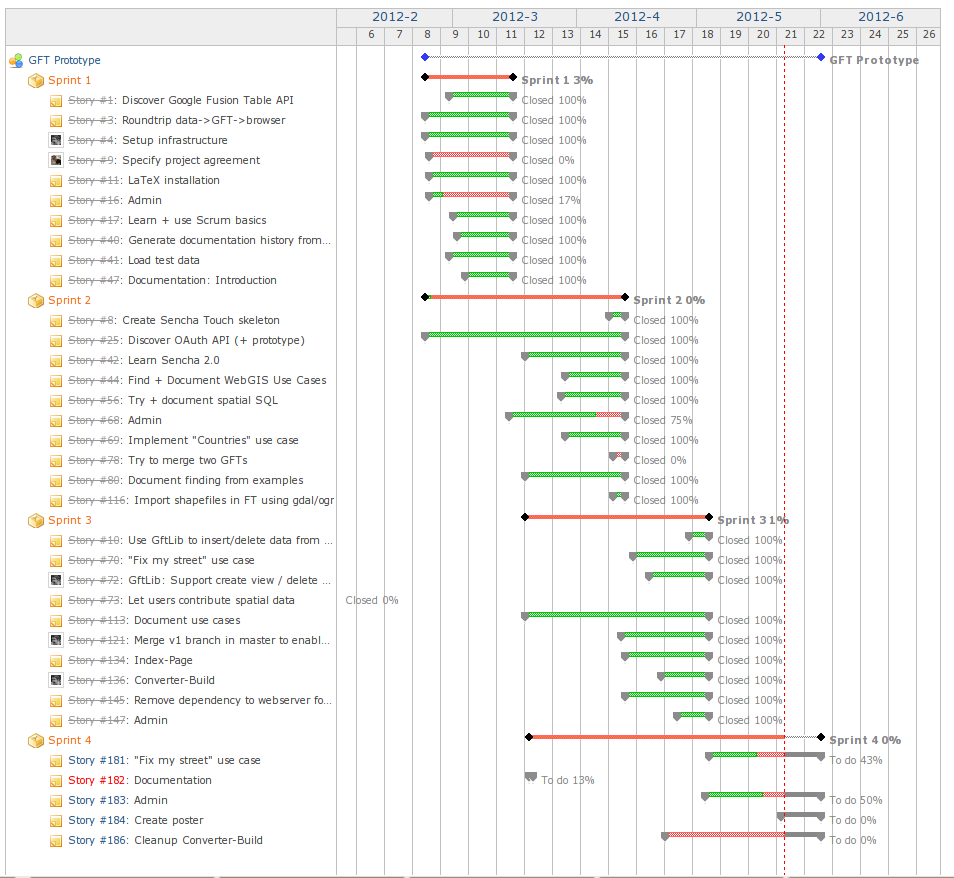
\includegraphics[width=\textwidth]{images/projektmanagement/overall_stories_gantt_chart}
	\caption{Gantt-Diagramm des Projektverlaufs}
	\label{overall_stories_gantt_chart}
\end{figure}

\subsection{Arbeitsaufwand}
Wie schon im Kapitel \ref{projektmanagement} beschrieben, war der vom Modul vorgegebene Aufwand pro Person auf 240h festgelegt. In Tabelle \ref{projektmanagement-arbeitsaufwand} ersichtlich haben wir diesen beide leicht überschritten.

\begin{longtable}{|l|l|}
\hline 
\textbf{Person} & \textbf{Aufwand} \\ 
\hline 
Stefan Oderbolz & 250h \\ 
\hline 
Jürg Hunziker & 260h \\ 
\hline 
\caption{Arbeitsaufwand pro Person}
\label{projektmanagement-arbeitsaufwand}
\end{longtable} 

\subsection{Fazit}
\todo[inline]{Projektverlauf Fazit schreiben}